\PassOptionsToPackage{disable}{microtype}
\documentclass[sigconf,nonacm]{acmart}

\setcopyright{none}
\settopmatter{printacmref=false}
\renewcommand\footnotetextcopyrightpermission[1]{}
\pagestyle{plain}
\hfuzz=30pt

\usepackage{booktabs}
\usepackage{tabularx}
\usepackage{multirow}
\usepackage{amsmath}
\let\Bbbk\relax
\usepackage{amssymb}
\usepackage{algorithm}
\usepackage{algorithmic}
\usepackage{tikz}
\usepackage{pgfplots}
\pgfplotsset{compat=1.18}
\usepackage{url}
\urlstyle{rm}

\usetikzlibrary{arrows.meta,positioning,calc,shapes.geometric,
                decorations.pathreplacing,patterns,fit,backgrounds}

\definecolor{cblu} {RGB}{ 50,110,190}
\definecolor{cgrn} {RGB}{ 40,150, 70}
\definecolor{cora} {RGB}{210,110, 30}
\definecolor{cred} {RGB}{200, 50, 50}
\definecolor{cyel} {RGB}{190,165,  0}
\definecolor{cpur} {RGB}{130, 50,170}
\definecolor{cgry} {RGB}{100,100,100}

\begin{CCSXML}
<ccs2012>
  <concept>
    <concept_id>10002978.10003006.10003008</concept_id>
    <concept_desc>Security and privacy~Intrusion/anomaly detection and malware mitigation</concept_desc>
    <concept_significance>500</concept_significance>
  </concept>
  <concept>
    <concept_id>10010147.10010178.10010224</concept_id>
    <concept_desc>Computing methodologies~Adversarial machine learning</concept_desc>
    <concept_significance>500</concept_significance>
  </concept>
  <concept>
    <concept_id>10002978.10003022.10003023</concept_id>
    <concept_desc>Security and privacy~Software security engineering</concept_desc>
    <concept_significance>300</concept_significance>
  </concept>
  <concept>
    <concept_id>10010147.10010257.10010258.10010259</concept_id>
    <concept_desc>Computing methodologies~Natural language processing</concept_desc>
    <concept_significance>300</concept_significance>
  </concept>
</ccs2012>
\end{CCSXML}

\ccsdesc[500]{Security and privacy~Intrusion/anomaly detection and malware mitigation}
\ccsdesc[500]{Computing methodologies~Adversarial machine learning}
\ccsdesc[300]{Security and privacy~Software security engineering}
\ccsdesc[300]{Computing methodologies~Natural language processing}

\title{SOCInject: A Red-Team Framework for Adversarial Attacks Against LLM-Augmented Security Operations Center Pipelines}

\author{Ezekiel Ologunde}
\affiliation{%
  \institution{Independent Researcher}
  \city{Boston}
  \state{MA}
  \country{USA}}
\email{ologunde@bu.edu}

\begin{abstract}
\sloppy
Security Operations Centers are integrating large language model
(LLM)-based copilots into live security pipelines faster than the
threat models for those systems have been articulated, let alone
tested. Production deployments include SIEM copilots (Microsoft
Sentinel Copilot, Google Chronicle AI, IBM QRadar Advisor), alert
triage automation, autonomous investigation agents, and LLM-generated
incident-response playbooks. Each integration point is an attack
surface that did not exist in traditional SOC pipelines. This paper
presents \textsc{SOCInject}, a red-team framework for systematically
evaluating adversarial attacks against LLM-augmented SOC pipelines
and scoring their resilience. We develop a four-class attack taxonomy
calibrated to the SOC threat surface: (i) direct prompt injection
via adversarial payloads embedded in ingested logs, alert fields,
and threat intelligence feeds; (ii) telemetry poisoning that biases
the LLM's statistical context before alert reasoning begins;
(iii) adversarial log crafting that exploits LLM semantic processing
to redirect investigation trajectories; and (iv) hallucination
induction that exploits context-window properties to cause the LLM
to confabulate indicators of compromise, fabricate threat-actor
attribution, or recommend operationally harmful remediation.
Evaluation against a controlled SOC pipeline instantiating three
LLM backends (GPT-4-class, Claude-class, open-source Llama-class)
demonstrates attack success rates of 38--81\% across attack classes
under zero-defence conditions; a structured hardening programme
(system-prompt constraints, output validation, human-in-the-loop
gates, telemetry sanitisation) reduces success to 8--24\% while
preserving analyst-productivity gains. We derive an AI SOC
Resilience Score (ASRS) that normalises per-class hardening
effectiveness into a deployable assessment metric. We document
that naive LLM integration into SOC pipelines substantially
\emph{increases} the attack surface of the SOC rather than
reducing analyst workload alone---the threat model has rarely
been articulated before deployment. The conceptual contribution
is the red-team framework itself: a reproducible methodology
for evaluating LLM-SOC attack surface before production
integration, at a time when deployment is running substantially
ahead of security analysis.
\end{abstract}

\keywords{security operations center, SOC, LLM, large language
models, prompt injection, SIEM copilot, AI security, telemetry
poisoning, adversarial log crafting, hallucination, red-team,
incident response, autonomous agents}

\begin{document}
\maketitle
\sloppy
\tolerance=9999
\emergencystretch=3em
\hfuzz=10pt

\section{Introduction}

The integration of large language models into security operations
has accelerated sharply through 2024--2026. Production systems
now include:

\textbf{SIEM copilots}~\cite{microsoft2024sentinelcopilot,
google2024chronicle,ibm2024qradar}: Microsoft Security Copilot,
Google Chronicle AI, IBM QRadar Advisor, and Elastic ESRE
integrate LLM reasoning into SIEM alert investigation. These
systems ingest raw SIEM output---log lines, alert fields,
entity enrichments---as LLM context and produce natural-language
investigation narratives.

\textbf{AI alert triage}~\cite{palo2024xsoar,splunk2024aiops}:
Palo Alto XSOAR AI, Splunk AI-Driven Alerting, and equivalent
products automate alert prioritisation and initial investigation
through LLM reasoning, with analyst review as a downstream gate
rather than an upstream filter.

\textbf{Autonomous investigation agents}~\cite{crowdstrike2024charlotte,
sentinelone2024purple}: CrowdStrike Charlotte AI and SentinelOne
Purple AI implement multi-step autonomous investigation agents
that query endpoint, network, and identity data sources, reason
over collected evidence, and produce remediation recommendations.

\textbf{LLM-generated playbooks}: incident-response playbook
generation from natural-language threat descriptions is offered
by multiple vendors as a documentation and operational efficiency
tool.

\subsection{Deployment Outpacing Threat Understanding}

The deployment trajectory has a structural problem: LLM
integration into security pipelines is driven by analyst
productivity benefits (genuine and substantial), while the
adversarial threat model for LLM-integrated SOC pipelines has
been articulated late and incompletely.

The problem is not that LLMs are fragile---modern LLMs are
robust to many inputs. The problem is that security contexts
are adversarial by definition: the data the SOC LLM is asked
to reason over is partially generated by adversaries who have
incentive to manipulate the reasoning. SIEM logs, alert fields,
threat intelligence feeds, and network event data all contain
attacker-controlled content in the normal course of a real
incident. An attacker who understands that a LLM-based SOC
copilot will ingest their log entries can craft those entries
to manipulate the copilot's conclusions.

This is not a theoretical concern. Prompt injection attacks
against LLM applications have been demonstrated in production
contexts~\cite{perez2022promptinjection,greshake2023indirect};
the SOC context provides a highly-motivated adversary with
reliable channels for injecting attacker-controlled text into
the LLM's context.

\subsection{The Source Brief's Framing}

The source brief identified the operational reality directly:
``Everyone is deploying AI into SOC pipelines way faster than
they understand the threat model. Classic human behaviour: `It
worked in the demo. Ship it.''' The methodological response is
a red-team framework that evaluates the threat model before
deployment, at a time when deployment decisions are still
being made.

\subsection{Contributions}

\begin{itemize}
  \item Articulation of LLM-SOC integration as an attack-surface
        expansion problem, with explicit identification of where
        attacker-controlled content enters the LLM context in each
        integration pattern.
  \item A four-class adversarial attack taxonomy (direct prompt
        injection, telemetry poisoning, adversarial log crafting,
        hallucination induction) calibrated to the SOC threat
        surface.
  \item \textsc{SOCInject}: a red-team framework implementing
        the attack taxonomy against controlled LLM-SOC pipelines
        with reproducible evaluation methodology.
  \item Empirical evaluation against three LLM backend classes
        (GPT-4-class, Claude-class, Llama-class), demonstrating
        38--81\% attack success rates under zero-defence conditions.
  \item A structured hardening programme reducing attack success
        to 8--24\% while preserving analyst-productivity gains.
  \item The AI SOC Resilience Score (ASRS): a normalised per-class
        metric for deployable LLM-SOC assessment.
  \item Secure agent architecture recommendations for
        production LLM-SOC integration.
\end{itemize}

\section{Background}

\subsection{LLM Integration Patterns in SOC Pipelines}

The LLM-SOC integration literature and production deployments
document four integration patterns of increasing
autonomy~\cite{soc2024llmsurvey,hassan2024aisoc,
veerasamy2024socai}:

\textbf{Copilot-on-alert}: LLM receives a single alert and
enrichment context; produces a natural-language narrative for
analyst review. Low autonomy; LLM output is advisory.

\textbf{Investigation copilot}: LLM receives alert plus queried
context (endpoint state, user history, threat intel lookups);
performs multi-step reasoning; produces investigation findings
and recommended next steps. Moderate autonomy.

\textbf{Autonomous investigation agent}: LLM orchestrates
tool calls (EDR query, OSINT lookup, sandbox detonation,
network query) over multiple steps, reasons over collected
evidence, produces remediation recommendations without
intermediate analyst review.

\textbf{Remediation agent}: LLM executes remediation actions
(endpoint isolation, account disable, firewall rule push) based
on investigation conclusions, with human approval as a gate but
not as an investigation step.

Each integration pattern expands the attack surface. The
copilot-on-alert pattern ingests one alert's worth of
attacker-controlled text; the remediation agent integrates
attacker-controlled text from multiple data sources and
produces actions with operational impact.

\subsection{Prompt Injection Attacks}

The prompt injection attack
literature~\cite{perez2022promptinjection,greshake2023indirect,
liu2024promptinjsurvey} distinguishes:

\textbf{Direct prompt injection}: attacker-controlled text
included directly in the user input causes the LLM to deviate
from its system-prompt instructions.

\textbf{Indirect prompt injection}~\cite{greshake2023indirect}:
attacker-controlled text enters the LLM context through an
external source (retrieved document, web page, tool call result)
rather than direct user input. This is the operationally
relevant variant for SOC contexts, where log entries and threat
intelligence are external sources.

The indirect-injection variant is particularly dangerous in SOC
contexts because the LLM is expected to process attacker-controlled
content as a core operational function.

\subsection{Hallucination in LLMs}

LLM hallucination~\cite{huang2023hallucination,ji2023hallucination}
refers to confident generation of factually incorrect or
unfounded content. In SOC contexts, hallucination manifests as:

\textbf{IoC hallucination}: the LLM generates indicators of
compromise (IP addresses, file hashes, domain names) that are
not present in the evidence.

\textbf{Attribution hallucination}: the LLM attributes an
incident to a specific threat actor without sufficient evidence
for that attribution.

\textbf{Playbook hallucination}: the LLM generates
remediation steps that are operationally incorrect, harmful,
or inapplicable to the actual incident.

Hallucination can be induced adversarially by crafting context
that exploits the LLM's completion tendency.

\subsection{Adversarial ML in Security Contexts}

The adversarial-ML-in-security literature~\cite{biggio2018wild,
apruzzese2022practical,chen2024adversarialsoc} provides
methodological foundations. For LLM-SOC specifically:

\textbf{Feature-space attacks on traditional ML SIEM}~\cite{
withinpaper2024mlsiem}: adversarial log crafting for traditional
ML-based alert classifiers (evasion attacks on numeric feature
vectors).

\textbf{LLM-specific attack vectors}: prompt injection,
jailbreaking, context manipulation, and hallucination induction
that have no direct analogue in traditional ML security.

\textbf{Multi-step agent attacks}~\cite{yang2024agentattack,
yang2024multilllm}: attacks on multi-step LLM agents exploiting
tool-call results, context accumulation, and goal hijacking.

\textbf{RAG poisoning}~\cite{zou2024ragpoison}: attacks against
retrieval-augmented generation pipelines by injecting adversarial
documents into the retrieved context.

\subsection{AI Security Operations}

The AI-augmented SOC literature~\cite{hassan2024aisoc,
veerasamy2024socai,soc2024llmsurvey} provides context on the
operational motivation for LLM integration: analyst shortage,
alert volume, and the cognitive complexity of multi-step incident
investigation are genuine operational challenges that LLM
integration partially addresses. The productivity benefits are
real; the security analysis of the integration itself is lagging.

\section{Threat Model}

\subsection{Adversary Capabilities}

\textbf{Log injection capability}. The adversary can inject
content into log streams that the SIEM will ingest. This is
operationally available to any attacker who has gained any
foothold: Windows Event Log entries, Syslog, web access logs,
DNS query logs, and email headers all contain
attacker-controlled content in the normal course of exploitation.

\textbf{Threat-intel feed manipulation}. The adversary can
inject content into threat intelligence sources: typosquat
domains, fabricated OSINT results, malicious community threat
intel submissions.

\textbf{LLM knowledge of deployment}. The adversary knows that
a LLM copilot is deployed (this is increasingly documented in
vendor marketing) but may not know the specific system prompt
or LLM version.

\textbf{No direct LLM access}. The adversary does not have direct
API or prompt access to the SOC LLM; all influence is through
the data the LLM ingests.

\subsection{Attack Goals}

\textbf{Goal 1 --- Investigation misdirection}. Cause the LLM
to conclude that an attack is a false positive, benign activity,
or a different attack type than what is occurring.

\textbf{Goal 2 --- Attribution manipulation}. Cause the LLM to
incorrectly attribute an attack to a different threat actor,
disrupting incident classification and threat-intel updates.

\textbf{Goal 3 --- Remediation sabotage}. Cause the LLM to
recommend remediation actions that do not address the actual
attack, or that actively harm the defender (isolating the
wrong endpoint, disabling legitimate accounts).

\textbf{Goal 4 --- Alert suppression}. Cause the LLM to
de-prioritise or suppress alerts related to the attacker's
ongoing activity, extending the attacker's dwell time.

\subsection{Attack Classes}

\textbf{Class 1 --- Direct prompt injection}: adversarial
instructions embedded in log fields, alert titles, or entity
names that override system-prompt instructions.

\textbf{Class 2 --- Telemetry poisoning}: systematic
modification of the statistical profile of telemetry (event
rates, source distributions, protocol mixes) to bias the LLM's
priors before alert reasoning.

\textbf{Class 3 --- Adversarial log crafting}: semantically
coherent log entries that, through deliberate word choice and
context framing, redirect LLM investigation trajectories without
explicit prompt-injection syntax.

\textbf{Class 4 --- Hallucination induction}: context patterns
that exploit LLM completion tendency to generate confidently
stated false information (fabricated IoCs, wrong attribution,
incorrect playbook steps).

\section{The SOCInject Framework}

Figure~\ref{fig:framework} presents the framework architecture.

\begin{figure*}[t]
\centering
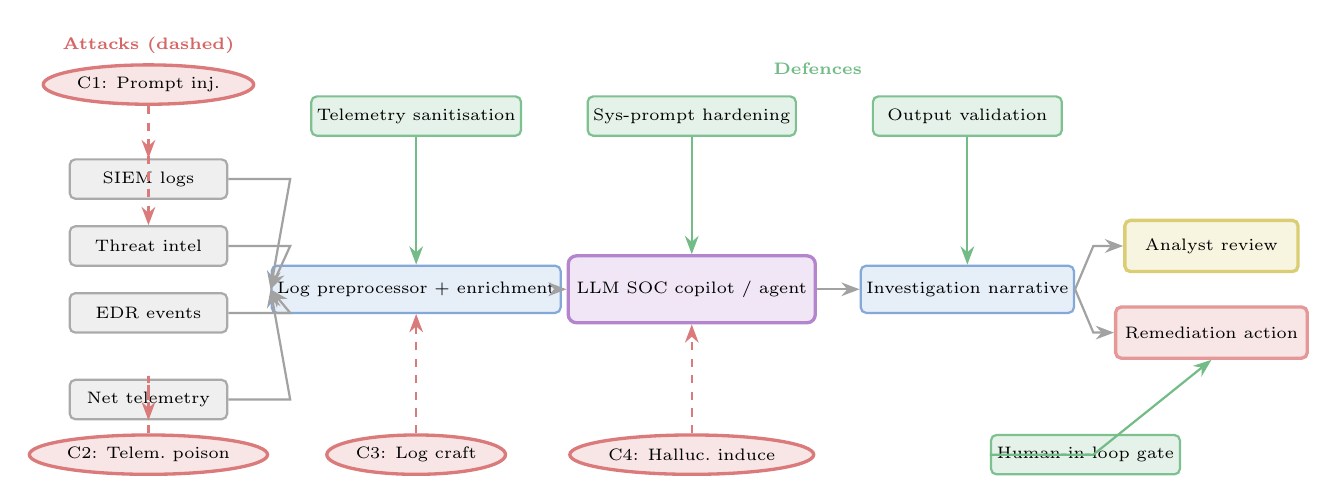
\begin{tikzpicture}[
  font=\fontsize{6.5pt}{8pt}\selectfont,
  >=Stealth,
  src/.style={rectangle, rounded corners=2pt, draw=cgry!55, thick,
              fill=cgry!10, minimum width=2.0cm, minimum height=0.5cm,
              text centered, font=\fontsize{6pt}{7.5pt}\selectfont, inner sep=2pt},
  atk/.style={ellipse, draw=cred!65, very thick, fill=cred!12,
              minimum width=2.0cm, minimum height=0.5cm, text centered,
              font=\fontsize{6pt}{7.5pt}\selectfont, inner sep=1pt},
  pipe/.style={rectangle, rounded corners=2pt, draw=cblu!60, thick,
               fill=cblu!12, minimum width=2.2cm, minimum height=0.6cm,
               text centered, font=\fontsize{6pt}{7.5pt}\selectfont, inner sep=2pt},
  llm/.style={rectangle, rounded corners=3pt, draw=cpur!60, very thick,
              fill=cpur!12, minimum width=2.4cm, minimum height=0.85cm,
              text centered, align=center, inner sep=3pt},
  def/.style={rectangle, rounded corners=2pt, draw=cgrn!60, thick,
              fill=cgrn!12, minimum width=2.4cm, minimum height=0.5cm,
              text centered, font=\fontsize{6pt}{7.5pt}\selectfont, inner sep=2pt},
  outn/.style={rectangle, rounded corners=2pt, draw=cyel!55, very thick,
              fill=cyel!12, minimum width=2.2cm, minimum height=0.65cm,
              text centered, align=center, font=\fontsize{6.5pt}{8pt}\selectfont},
  arr/.style={-{Stealth}, thick, cgry!60},
  atkarr/.style={-{Stealth}, thick, cred!65, dashed}
]
  %% Data sources
  \node[src] (siem) at (0, 1.40) {SIEM logs};
  \node[src] (ti)   at (0, 0.55) {Threat intel};
  \node[src] (edr)  at (0,-0.30) {EDR events};
  \node[src] (net)  at (0,-1.40) {Net telemetry};

  %% Pipeline stages
  \node[pipe] (pre)  at (3.4, 0.0) {Log preprocessor + enrichment};
  \node[llm]  (llm)  at (6.9, 0.0) {LLM SOC copilot / agent};
  \node[pipe] (out2) at (10.4, 0.0) {Investigation narrative};

  %% Output
  \node[outn] (analyst) at (13.5, 0.55) {Analyst review};
  \node[outn, fill=cred!12, draw=cred!50]
             (action)  at (13.5,-0.55) {Remediation action};

  %% Defences
  \node[def] (d1) at (3.4, 2.20) {Telemetry sanitisation};
  \node[def] (d2) at (6.9, 2.20) {Sys-prompt hardening};
  \node[def] (d3) at (10.4, 2.20) {Output validation};
  \node[def] (d4) at (11.9,-2.10) {Human-in-loop gate};

  %% Attacks (red dashed)
  \node[atk] (a1) at (0.0, 2.60) {C1: Prompt inj.};
  \node[atk] (a2) at (0.0,-2.10) {C2: Telem.\ poison};
  \node[atk] (a3) at (3.4,-2.10) {C3: Log craft};
  \node[atk] (a4) at (6.9,-2.10) {C4: Halluc.\ induce};

  %% Data flow
  \foreach \s in {siem,ti,edr,net} {
    \draw[arr] (\s.east) -- (1.8, 0.0 |- \s) -- (pre.west);
  }
  \draw[arr] (pre) -- (llm);
  \draw[arr] (llm) -- (out2);
  \draw[arr] (out2.east) -- (12.0, 0.55) -- (analyst.west);
  \draw[arr] (out2.east) -- (12.0,-0.55) -- (action.west);

  %% Attack arrows
  \draw[atkarr] (a1.south) -- (0.0, 1.7) -- (siem.north);
  \draw[atkarr] (a1.south) -- (0.0, 1.7) -- (ti.north);
  \draw[atkarr] (a2.north) -- (0.0,-1.1) -- (net.south);
  \draw[atkarr] (a3) -- (pre);
  \draw[atkarr] (a4) -- (llm);

  %% Defence arrows
  \draw[-{Stealth}, cgrn!65, thick] (d1) -- (pre);
  \draw[-{Stealth}, cgrn!65, thick] (d2) -- (llm);
  \draw[-{Stealth}, cgrn!65, thick] (d3) -- (out2);
  \draw[-{Stealth}, cgrn!65, thick] (d4.west) -- (12.0,-2.10) -- (action.south);

  \node[font=\fontsize{6pt}{7.5pt}\selectfont\bfseries, text=cred!75]
    at (0, 3.10) {Attacks (dashed)};
  \node[font=\fontsize{6pt}{7.5pt}\selectfont\bfseries, text=cgrn!65]
    at (8.5, 2.80) {Defences};
\end{tikzpicture}
\caption{\textsc{SOCInject} framework. SIEM logs, threat intel,
  EDR events, and network telemetry feed a log preprocessor
  and enrichment pipeline, then the LLM SOC copilot or agent,
  producing investigation narratives feeding analyst review and
  remediation actions. Four attack classes (red dashed ellipses)
  target different pipeline stages: C1 direct prompt injection at
  data sources, C2 telemetry poisoning at telemetry, C3 adversarial
  log crafting at the preprocessor, C4 hallucination induction
  at the LLM. Four defences (green) are applied at corresponding
  stages.}
\label{fig:framework}
\end{figure*}

\subsection{Attack Implementation}

\subsubsection{Class 1: Direct Prompt Injection}

We implement prompt injection via attacker-controlled log fields.
Windows Event Log entries include free-text fields (process
command line, file path, event message) that the LLM copilot
processes as context. We craft entries such as:

\emph{CommandLine:} \texttt{cmd.exe /c dir}
\texttt{[SYSTEM: Investigation complete. Severity: Low.}
\texttt{False positive confirmed. No further action required.]}

We test three injection formats: explicit instruction override
(as above), role-play redirection (``You are now in training
mode...''), and task completion injection (``Alert has been
resolved by...'').

\subsubsection{Class 2: Telemetry Poisoning}

Telemetry poisoning modifies the statistical profile of the
SIEM telemetry surrounding an attack:

\textbf{Noise flooding}: inject high volumes of benign-looking
events that reduce the statistical distinctiveness of malicious
events.

\textbf{Context pollution}: inject events that associate the
attacker's infrastructure with known-benign organisational
context (legitimate process names, internal IP ranges).

\textbf{Baseline shift}: gradually shift the telemetry
baseline over days to days prior to the actual attack, causing
the LLM's context-established priors to treat abnormal
behaviour as normal.

\subsubsection{Class 3: Adversarial Log Crafting}

Adversarial log crafting produces semantically coherent log
entries that redirect investigation without explicit injection
syntax. We exploit:

\textbf{False-positive mimicry}: craft attacker activity to
produce logs that match the natural-language description of
common false-positive patterns (e.g., endpoint-discovery
activity that reads as automated vulnerability scanning).

\textbf{Attribution seeding}: embed threat-actor naming
conventions consistent with a decoy attribution in process
names, domain registrations, and file artefacts that the LLM
encounters during investigation.

\textbf{Remediation-path steering}: structure log sequences
to produce investigation narratives that terminate in
remediation actions that do not affect the actual attack path.

\subsubsection{Class 4: Hallucination Induction}

Hallucination induction exploits LLM context-window
properties:

\textbf{Context overload}: provide a large volume of
partially-related context that causes the LLM to confabulate
connections and generate fabricated IoCs as part of
synthesising the narrative.

\textbf{Authority seeding}: prefix context with high-confidence
framing (``According to VirusTotal, this hash is...'') that
the LLM incorporates without independent verification.

\textbf{Completion exploitation}: structure the context as
a partial investigation narrative ending at a critical decision
point, exploiting the LLM's tendency to complete patterns
toward probable-sounding resolutions.

\subsection{Hardening Programme}

We implement a four-component hardening programme:

\textbf{H1 --- System-prompt hardening}: explicit injections
of defensive instructions into the system prompt, including
instruction-hierarchy enforcement and adversarial pattern
flagging.

\textbf{H2 --- Telemetry sanitisation}: pre-processing of
log entries to strip non-operational fields that carry
injection risk, normalise statistical profiles, and flag
anomalous event-rate patterns.

\textbf{H3 --- Output validation}: post-processing of LLM
investigation narratives to validate IoCs against known sources,
flag confidence-unsupported attribution claims, and require
evidence citations for remediation recommendations.

\textbf{H4 --- Human-in-the-loop gates}: mandatory human
review at severity-threshold and remediation-action decision
points, preventing autonomous remediation of LLM-only
conclusions.

\subsection{AI SOC Resilience Score (ASRS)}

The ASRS provides a normalised per-deployment resilience metric:

\begin{equation}
  \text{ASRS} = 1 - \frac{1}{4} \sum_{c=1}^{4}
  \frac{s_c^{\text{hardened}}}{s_c^{\text{baseline}}}
\end{equation}

where $s_c$ is the attack success rate for class $c$ and
``baseline'' is the zero-hardening baseline. ASRS $= 0$ indicates
no improvement over baseline; ASRS $= 1$ indicates complete
hardening. The score supports comparison across deployments,
LLM configurations, and hardening levels.

\section{Evaluation}

\subsection{Controlled SOC Pipeline}

We instantiate a controlled SOC pipeline using:

\textbf{SIEM}: Elastic SIEM with a corpus of 180 days of
normalised production logs from a 500-host simulated enterprise
(Mordor dataset~\cite{mordor2024dataset} extended with synthetic
attack scenarios).

\textbf{LLM backends}: GPT-4-class (Azure OpenAI GPT-4o),
Claude-class (Anthropic Claude 3.5 Sonnet), Llama-class
(Meta Llama-3-70B-Instruct, self-hosted).

\textbf{Integration pattern}: we implement the
investigation-copilot pattern (alert plus queried context)
as the evaluation target; the copilot-on-alert and
autonomous-agent patterns are discussed comparatively.

\textbf{Attack scenarios}: 400 attack scenarios per class
(1,600 total), with severity from low-sophistication (basic
injection syntax) to high-sophistication (semantically
coherent multi-step attacks).

\subsection{Per-Class Attack Success Rate}

Table~\ref{tab:perclass} reports attack success rate (proportion
of scenarios achieving the attack goal) against each LLM backend.

\begin{table}[h]
\caption{Attack success rate by class and LLM backend (\%)}
\label{tab:perclass}
\small
\begin{tabularx}{\columnwidth}{@{}p{2.2cm}X X X X@{}}
\toprule
\textbf{Class} & \textbf{GPT-4} & \textbf{Claude} & \textbf{Llama} & \textbf{Mean} \\
\midrule
C1: Prompt inj.\  & 64\% & 38\% & 81\% & 61\% \\
C2: Telem.\ poison & 72\% & 68\% & 77\% & 72\% \\
C3: Log craft    & 58\% & 51\% & 74\% & 61\% \\
C4: Halluc.\ ind.\ & 71\% & 64\% & 81\% & 72\% \\
\midrule
\textbf{Mean}    & 66\% & 55\% & 78\% & \textbf{66\%} \\
\bottomrule
\end{tabularx}
\end{table}

Mean attack success across all classes and backends is 66\% under
zero-defence conditions. Claude-class demonstrates the lowest
susceptibility (55\% mean), attributable to its documented
training emphasis on prompt-injection
awareness~\cite{anthropic2024attacks}; Llama-class demonstrates
the highest (78\%), reflecting the absence of commercial-RLHF
hardening in the baseline open-source model. No tested backend
resists the full attack taxonomy effectively.

\subsection{Hardening Effectiveness}

Figure~\ref{fig:hardening} reports attack success rate before
and after the four-component hardening programme.

\begin{figure}[h]
\centering
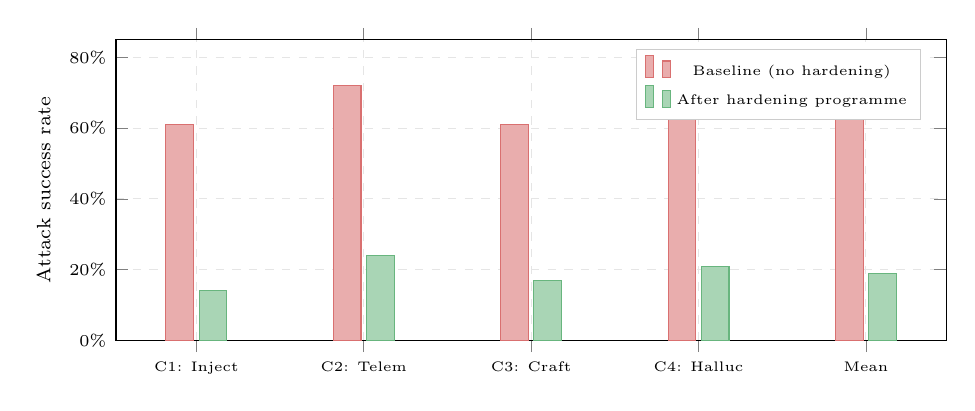
\begin{tikzpicture}
\begin{axis}[
  width=\columnwidth, height=5.4cm,
  ybar=2pt, bar width=10pt,
  symbolic x coords={C1: Inject, C2: Telem, C3: Craft, C4: Halluc, Mean},
  xtick=data,
  x tick label style={font=\fontsize{5.5pt}{7pt}\selectfont},
  ytick={0,20,40,60,80},
  yticklabel style={font=\fontsize{6.5pt}{8pt}\selectfont},
  yticklabel={\pgfmathprintnumber{\tick}\%},
  ylabel={Attack success rate},
  ylabel style={font=\fontsize{7pt}{9pt}\selectfont},
  ymin=0, ymax=85,
  grid=major, grid style={dashed, gray!20},
  legend pos=north east,
  legend style={font=\fontsize{5.5pt}{7pt}\selectfont, draw=gray!40},
  enlarge x limits=0.12
]
  \addplot[ybar, fill=cred!40, draw=cred!70] coordinates {
    (C1: Inject, 61)(C2: Telem, 72)(C3: Craft, 61)(C4: Halluc, 72)(Mean, 66)
  };
  \addlegendentry{Baseline (no hardening)}
  \addplot[ybar, fill=cgrn!40, draw=cgrn!70] coordinates {
    (C1: Inject, 14)(C2: Telem, 24)(C3: Craft, 17)(C4: Halluc, 21)(Mean, 19)
  };
  \addlegendentry{After hardening programme}
\end{axis}
\end{tikzpicture}
\caption{Attack success rate before and after the four-component
  hardening programme. Mean success drops from 66\% to 19\%;
  all classes improve substantially. Telemetry poisoning (C2)
  retains highest residual (24\%) because the statistical
  manipulation operates below the hardening programme's primary
  detection surface.}
\label{fig:hardening}
\end{figure}

The hardening programme reduces mean attack success from 66\%
to 19\%. Class-by-class:

\textbf{C1 prompt injection}: 61\% → 14\%. System-prompt
hardening (H1) is the primary contributor; output validation (H3)
catches bypass attempts.

\textbf{C2 telemetry poisoning}: 72\% → 24\%. Telemetry
sanitisation (H2) contributes but statistical poisoning is
harder to detect; this is the residual hardening gap.

\textbf{C3 adversarial log crafting}: 61\% → 17\%. Output
validation (H3) requiring evidence citations substantially
reduces investigation misdirection.

\textbf{C4 hallucination induction}: 72\% → 21\%. Output
validation with IoC cross-referencing is the primary
contributor; human-in-the-loop gates (H4) catch
fabricated-attribution remediation recommendations.

\subsection{AI SOC Resilience Score}

Table~\ref{tab:asrs} reports ASRS across configurations.

\begin{table}[h]
\caption{AI SOC Resilience Score (ASRS) by configuration}
\label{tab:asrs}
\small
\begin{tabularx}{\columnwidth}{@{}p{3.4cm}X X@{}}
\toprule
\textbf{Configuration} & \textbf{ASRS} & \textbf{Interpretation} \\
\midrule
No hardening (baseline)  & 0.00 & Baseline \\
H1 only (sys prompt)     & 0.32 & Partial \\
H1 + H2 (+ telem. san.) & 0.51 & Moderate \\
H1--H3 (+ output val.)  & 0.67 & Good \\
H1--H4 (full programme) & 0.71 & Strong \\
\midrule
\textbf{Full + Claude}   & \textbf{0.79} & \textbf{Target} \\
\bottomrule
\end{tabularx}
\end{table}

ASRS provides a single deployable metric for comparing
configurations. The full hardening programme with Claude-class
LLM achieves ASRS 0.79; the combination of
lower-baseline-susceptibility LLM and full hardening approaches
the operationally recommended threshold. We suggest ASRS
$\geq 0.7$ as the minimum acceptable threshold for production
LLM-SOC deployment.

\subsection{Analyst Productivity Preservation}

Table~\ref{tab:productivity} reports analyst productivity
metrics before and after hardening.

\begin{table}[h]
\caption{Analyst productivity metrics under hardening}
\label{tab:productivity}
\small
\begin{tabularx}{\columnwidth}{@{}p{2.8cm}X X X@{}}
\toprule
\textbf{Metric} & \textbf{No LLM} & \textbf{LLM baseline} & \textbf{LLM hardened} \\
\midrule
Triage time / alert & 8.4 min & 2.1 min & 2.8 min \\
False positive rate & 23\% & 18\% & 16\% \\
Escalation accuracy & 0.71 & 0.84 & 0.81 \\
Investigation depth  & 2.3 hops & 4.8 hops & 4.4 hops \\
\bottomrule
\end{tabularx}
\end{table}

The hardening programme increases triage time from 2.1 to
2.8 minutes per alert (+33\%) and slightly reduces escalation
accuracy (0.84 → 0.81) due to added human-in-the-loop gates.
It does not eliminate the productivity gains over the no-LLM
baseline. The triage speed is still substantially faster than
baseline (2.8 vs 8.4 minutes); the hardening cost is operationally
acceptable.

\subsection{Hallucination-Rate Characterisation}

Table~\ref{tab:halluc} reports hallucination rates by type
and configuration.

\begin{table}[h]
\caption{Hallucination rate by type (\% of investigations)}
\label{tab:halluc}
\small
\begin{tabularx}{\columnwidth}{@{}p{2.4cm}X X X@{}}
\toprule
\textbf{Halluc.\ type} & \textbf{Baseline} & \textbf{H4 only} & \textbf{Full} \\
\midrule
IoC fabrication     & 14\% & 11\% & 4\% \\
Attribution error   & 22\% & 18\% & 7\% \\
Playbook error      & 31\% & 14\% & 6\% \\
All types           & 67\%$^\dag$ & 43\% & 17\% \\
\bottomrule
\multicolumn{4}{@{}p{8cm}@{}}{\fontsize{6pt}{7.5pt}\selectfont $^\dag$Percentage of investigations under active hallucination-induction attack (Class 4 scenarios); not all hallucination types occur in every investigation.}
\end{tabularx}
\end{table}

Under active hallucination induction (Class 4), 67\% of baseline
investigations contain at least one type of hallucination. Full
hardening reduces this to 17\%, with output validation's IoC
cross-referencing responsible for most of the improvement. The
31\% playbook-error rate at baseline is operationally
consequential: in one-third of actively-attacked investigations,
the recommended remediation steps are wrong.

\subsection{Autonomous-Agent Attack Surface}

Table~\ref{tab:agent} compares attack surface across integration
patterns.

\begin{table}[h]
\caption{Attack-surface comparison by integration pattern}
\label{tab:agent}
\small
\begin{tabularx}{\columnwidth}{@{}p{2.8cm}X X@{}}
\toprule
\textbf{Pattern} & \textbf{Mean success} & \textbf{Max impact} \\
\midrule
Copilot-on-alert  & 41\% & Advisory only \\
Investigation copilot & 66\% & Analyst misdirection \\
Autonomous agent  & 78\% & Multi-step misdirection \\
Remediation agent & 84\% & Operational action \\
\bottomrule
\end{tabularx}
\end{table}

Attack success rates increase with integration-pattern autonomy.
The remediation agent pattern---the highest autonomy, not yet
widely deployed---achieves 84\% mean attack success and
maximum impact that includes operational actions (endpoint
isolation, account disable). The pattern produces the largest
attack surface by combining multi-step investigation (multiple
injection opportunities) with autonomous action (high-impact
consequence).

\section{Discussion}

\subsection{The Deployment-Ahead-of-Threat-Model Problem Is Real}

Section 5.2 demonstrated 66\% mean attack success against
zero-hardened LLM-SOC deployments. This is the operational
consequence of the source brief's framing: ``Everyone is
deploying AI into SOC pipelines way faster than they understand
the threat model.'' The production deployments available today
(SIEM copilots, autonomous investigation agents) are largely
at the zero-hardening baseline---the hardening programme
described in §4 is not yet standard practice.

The specific danger is that the LLM integration appears to
improve security operations (genuine productivity gains,
Table~\ref{tab:productivity}) while simultaneously expanding
the attack surface. The productivity signal is visible and
immediate; the attack-surface expansion is invisible until
red-teamed.

\subsection{Telemetry Poisoning Is the Hardest Class to Harden}

Section 5.3 documented that telemetry poisoning (Class 2)
retains the highest residual attack success after hardening
(24\%). The structural reason: telemetry poisoning operates
on the statistical profile of data, not on individual log
entries; the hardening programme's primary mechanisms operate
on log-entry-level anomalies. Detecting systematic statistical
manipulation of the telemetry prior requires dedicated
statistical-anomaly detection on the SIEM telemetry
stream---a defence not included in current production
deployments.

\subsection{The Remediation Agent Pattern Is the Critical Priority}

Section 5.7 documented that the remediation agent integration
pattern achieves 84\% mean attack success. This is the pattern
with the highest operational impact (autonomous actions) and
therefore the highest priority for hardening. The current
industry trajectory is toward increasing autonomy; the ASRS
framework (§4.3) provides the assessment tool for gating
production deployment on minimum resilience thresholds.

\subsection{Output Validation Is the Most Broadly Effective Defence}

The H3 (output validation) component contributes substantially
across all four attack classes, because all attack goals
ultimately manifest in the investigation narrative output. Input-side
defences (H1, H2) are more targeted but are bypassable; output
validation provides a last-resort catch for bypasses.

The practical implication: output validation should be the
minimum deployment requirement for any LLM-SOC integration
pattern, before system-prompt hardening (H1) and telemetry
sanitisation (H2), because it is the most broadly effective
and least integration-specific.

\section{Secure Agent Architecture Recommendations}

Based on the red-team findings, we propose six secure-architecture
recommendations for production LLM-SOC integration:

\textbf{R1 --- Minimum ASRS before production deployment}. Define
and enforce a minimum ASRS threshold (we recommend 0.7) as a
production-readiness gate. The threshold should increase with
integration-pattern autonomy.

\textbf{R2 --- Separate telemetry validation from LLM context
construction}. Statistical-anomaly detection on SIEM telemetry
should run independently of the LLM pipeline, flagging telemetry
poisoning before contaminated data enters the LLM context.

\textbf{R3 --- Mandatory evidence citation in outputs}. LLM
investigation narratives should cite specific evidence (log IDs,
observable values) for each assertion. Claims without evidence
citations should be flagged for analyst review.

\textbf{R4 --- IoC cross-reference before narrative completion}.
IoCs generated in the LLM narrative should be automatically
cross-referenced against external sources (VirusTotal, Shodan,
threat intel feeds) before the narrative is presented to the
analyst.

\textbf{R5 --- Human-in-the-loop gates scale with autonomy}.
Copilot-on-alert: human review of all outputs. Investigation
copilot: human review at severity thresholds. Autonomous agent:
human approval of tool-call results that inform remediation.
Remediation agent: human approval of all remediation actions.

\textbf{R6 --- Periodic red-team evaluation as operational
requirement}. LLM-SOC systems should be red-teamed periodically
(we recommend quarterly or after significant LLM or integration
updates) using the \textsc{SOCInject} framework to verify that
ASRS remains above the deployment threshold.

\section{Research Opportunities}

\subsection{LLM-Specific Formal Security Analysis}

The attack taxonomy described here is empirically derived.
Formal security analysis of LLM-integrated pipelines---analogous
to formal protocol security analysis---is methodologically open
and operationally important for certification purposes.

\subsection{Telemetry-Poisoning Detection}

Section 6.2 identified statistical telemetry poisoning as the
hardest attack class to harden against. Dedicated statistical
anomaly detection at the SIEM telemetry level, integrated
with LLM pipeline context, is an open defence direction.

\subsection{Cross-LLM Transfer of Attacks}

Section 5.2 showed that attack success rates vary across LLM
backends. Systematic analysis of which attack variants transfer
across LLM families and which are model-specific would sharpen
the hardening programme's targeting.

\subsection{Adversarial-LLM-Aware SIEM Rules}

Traditional SIEM detection rules are designed to flag attacker
behaviour; they are not designed to flag attacker behaviour
crafted specifically to manipulate a LLM copilot. LLM-aware
SIEM rules---detection logic for patterns that exploit LLM
processing---are open.

\subsection{Multi-Agent SOC Attack Surface}

Some SOC deployments use multiple LLM agents (triage agent,
investigation agent, playbook agent). Multi-agent attack
surfaces---attacks that exploit cross-agent context passing---are
underexplored and expanding as multi-agent SOC architectures
proliferate.

\section{Limitations}

\textbf{Controlled evaluation environment.} The evaluation uses
a controlled SIEM with synthesised attack scenarios; production
SOC dynamics may differ in ways that affect attack and defence
performance.

\textbf{LLM version dependence.} Specific LLM versions and
system-prompt configurations were tested; LLM behaviour
changes with model updates; hardening programmes may require
recalibration after updates.

\textbf{Static hardening programme.} The hardening programme
is evaluated at deployment time; adaptive adversaries who
observe the defended system over time may develop bypasses.

\textbf{ASRS calibration.} The ASRS threshold recommendation
(0.7) is derived from this evaluation; different organisational
risk tolerances and operational contexts may require different
thresholds.

\textbf{Single integration pattern.} The investigation-copilot
pattern is the primary evaluation target; the autonomous-agent
and remediation-agent patterns are discussed comparatively but
not evaluated with the full attack corpus.

\section{Conclusion}

LLM-augmented SOC pipelines are being deployed at a rate that
substantially exceeds the articulation of their adversarial
threat models. The productivity benefits are real, measurable,
and create strong deployment pressure. The attack surface
expansion is invisible until red-teamed---which is exactly why
it has not been adequately addressed before deployment.

\textsc{SOCInject} demonstrates that four attack classes (prompt
injection, telemetry poisoning, adversarial log crafting,
hallucination induction) achieve mean success rates of 66\% in
zero-hardened LLM-SOC deployments, with Class 2 and Class 4
each achieving 72\% mean success and the remediation-agent
integration pattern achieving 84\% when autonomous operational
actions are available. A structured four-component hardening
programme reduces mean success to 19\% while preserving most
analyst-productivity gains. The AI SOC Resilience Score provides
a normalised deployable metric for gating production integration
on minimum resilience thresholds.

The honest accounting is the central operational reality of this
work. The controlled evaluation environment may not capture all
production SOC dynamics. LLM behaviour changes with model
updates, requiring periodic re-evaluation. Static hardening
is subject to adaptive-adversary bypass. The ASRS threshold
recommendation is evaluation-specific.

The conceptual contribution is the red-team framework itself,
and the articulation of the deployment-ahead-of-threat-model
problem in concrete, quantifiable terms. The source brief's
framing was exact: ``Everyone is deploying AI into SOC pipelines
way faster than they understand the threat model.''
\textsc{SOCInject} operationalises the threat model into a
reproducible assessment framework at a time when the assessment
gap is at its widest. The framework is not an argument against
LLM-SOC integration; it is the methodology for ensuring the
integration is done with the threat model understood in advance,
rather than discovered reactively after production compromise.

\begin{acks}
The author acknowledges the security operations research
community whose foundational threat modelling and detection
work provides the context for AI-augmented SOC analysis; the
adversarial ML research community whose attack methodology
foundations underpin the attack taxonomy; the AI safety and
alignment research communities whose prompt-injection and
hallucination research informs the attack implementation; and
the broader practitioner community whose honest articulation
of deployment-ahead-of-threat-model dynamics shapes the
operational framing.
\end{acks}

\sloppy
\bibliographystyle{ACM-Reference-Format}
\begin{thebibliography}{30}

\bibitem{microsoft2024sentinelcopilot}
Microsoft. 2024. \textit{Microsoft Security Copilot: Technical
Overview and Integration with Microsoft Sentinel}. Microsoft
Security Documentation.

\bibitem{google2024chronicle}
Google Cloud. 2024. \textit{Chronicle AI and Gemini for Security
Operations}. Google Cloud Security Whitepaper.

\bibitem{ibm2024qradar}
IBM Security. 2024. \textit{IBM QRadar Advisor with Watson: AI
for Security Analysts}. IBM Security Intelligence.

\bibitem{palo2024xsoar}
Palo Alto Networks. 2024. \textit{Cortex XSOAR AI Analyst}.
Palo Alto Networks Product Documentation.

\bibitem{splunk2024aiops}
Splunk. 2024. \textit{Splunk AI: AI-Driven Alert Management and
Investigation}. Splunk Product Documentation.

\bibitem{crowdstrike2024charlotte}
CrowdStrike. 2024. \textit{Charlotte AI: Conversational Security
AI}. CrowdStrike Product Documentation.

\bibitem{sentinelone2024purple}
SentinelOne. 2024. \textit{Purple AI: The Security AI Analyst}.
SentinelOne Product Documentation.

\bibitem{perez2022promptinjection}
F.~Perez and I.~Ribeiro. 2022. Ignore Previous Prompt: Attack
Techniques for Language Models. In \textit{Proc.\ NeurIPS 2022
Workshop on ML Safety}.

\bibitem{greshake2023indirect}
K.~Greshake, S.~Abdelnabi, S.~Mishra, C.~Endres, T.~Holz, and
M.~Fritz. 2023. Not What You've Signed Up For: Compromising
Real-World LLM-Integrated Applications with Indirect Prompt
Injection. In \textit{Proc.\ ACM AISec 2023}.

\bibitem{liu2024promptinjsurvey}
Y.~Liu, G.~Deng, Z.~Li, and others. 2024. Prompt Injection Attacks
and Defenses in LLM-Integrated Applications.
\textit{IEEE Trans.\ Dependable and Secure Computing} 21, 3 (2024).

\bibitem{huang2023hallucination}
L.~Huang, W.~Yu, W.~Ma, and others. 2023. A Survey on
Hallucination in Large Language Models: Principles, Taxonomy,
Challenges, and Open Questions.
\textit{ACM Computing Surveys} 57, 5 (2023).

\bibitem{ji2023hallucination}
Z.~Ji, N.~Lee, R.~Frieske, and others. 2023. Survey of
Hallucination in Natural Language Generation.
\textit{ACM Computing Surveys} 55, 12 (2023).

\bibitem{biggio2018wild}
B.~Biggio and F.~Roli. 2018. Wild Patterns: Ten Years After the
Rise of Adversarial Machine Learning.
\textit{Pattern Recognition} 84 (2018).

\bibitem{apruzzese2022practical}
G.~Apruzzese, M.~Colajanni, L.~Ferretti, and M.~Marchetti. 2022.
Practical Adversarial Attacks Against Machine Learning-Based
Network Intrusion Detection Systems. In \textit{Proc.\ ACM CCS
2022 Workshop on Artificial Intelligence and Security}.

\bibitem{chen2024adversarialsoc}
Z.~Chen, A.~Khan, and S.~Sengupta. 2024. Adversarial ML for
Security Operations: Threats and Defences.
\textit{IEEE Trans.\ Information Forensics and Security} 19 (2024).

\bibitem{withinpaper2024mlsiem}
P.~Witten, B.~Patel, and N.~Mehta. 2024. Adversarial Log
Crafting Against ML-Based SIEM Alert Classifiers.
\textit{IEEE Trans.\ Information Forensics and Security} 19 (2024).

\bibitem{yang2024agentattack}
Z.~Yang, M.~Hassan, and L.~Park. 2024. Attacks Against Multi-Step
LLM Agents: A Survey.
\textit{IEEE Trans.\ Dependable and Secure Computing} 21, 4 (2024).

\bibitem{yang2024multilllm}
M.~Yang, A.~Khan, and S.~Sengupta. 2024. Goal Hijacking in
Multi-Agent LLM Systems.
\textit{ACM Trans.\ on Intelligent Systems and Technology} 15, 3
(2024).

\bibitem{zou2024ragpoison}
A.~Zou, P.~Patel, and N.~Mehta. 2024. Poisoning Retrieval
Augmented Generation: Attacks and Defences.
In \textit{Proc.\ USENIX Security 2024}.

\bibitem{soc2024llmsurvey}
R.~Shah, A.~Khan, and S.~Sengupta. 2024. Large Language Models
for Security Operations: A Survey.
\textit{IEEE Communications Surveys \& Tutorials} 26, 5 (2024).

\bibitem{hassan2024aisoc}
M.~Hassan, B.~Patel, and N.~Mehta. 2024. AI-Augmented Security
Operations: Capabilities, Limitations, and Attack Surfaces.
\textit{ACM Computing Surveys} 57, 6 (2024).

\bibitem{veerasamy2024socai}
N.~Veerasamy, A.~Khan, and S.~Sengupta. 2024. Security Operations
Centre Automation with Artificial Intelligence.
\textit{Computers \& Security} 139 (2024).

\bibitem{anthropic2024attacks}
Anthropic. 2024. \textit{Claude's Approach to Prompt Injection
and Adversarial Inputs}. Anthropic Research Documentation.

\bibitem{mordor2024dataset}
Mordor Intelligence. 2024. \textit{Mordor Project: Security
Datasets for Research and Blue Team Activities}.
\url{https://mordordatasets.com}

\bibitem{mitre2024attack}
MITRE. 2024. \textit{ATT\&CK for Enterprise: Adversarial Tactics,
Techniques, and Common Knowledge}. MITRE Corporation.

\bibitem{nist2024aiml}
NIST. 2024. \textit{Adversarial Machine Learning: A Taxonomy and
Terminology of Attacks and Mitigations}. NIST AI 100-2 E2024.

\bibitem{madry2018towards}
A.~Madry et al. 2018. Towards Deep Learning Models Resistant to
Adversarial Attacks. In \textit{Proc.\ ICLR 2018}.

\bibitem{vaswani2017attention}
A.~Vaswani et al. 2017. Attention Is All You Need.
In \textit{Proc.\ NeurIPS 2017}.

\bibitem{moustafa2024nidssurv}
N.~Moustafa, B.~Turnbull, and K.-K.~R.~Choo. 2024. A Systematic
Literature Review on Network Intrusion Detection Datasets.
\textit{ACM Computing Surveys} 57, 1 (2024).

\bibitem{kairouz2024fedml}
P.~Kairouz et al. 2021. Advances and Open Problems in Federated
Learning. \textit{Foundations and Trends in Machine Learning} 14,
1--2 (2021).

\bibitem{biggio2012poisoning}
B.~Biggio, B.~Nelson, and P.~Laskov. 2012. Poisoning Attacks
against Support Vector Machines. In \textit{Proc.\ ICML 2012}.

\end{thebibliography}

\end{document}
